\documentclass[12pt,french,dvips]{report} 

%\usepackage[latin1]{inputenc}
\usepackage[utf8]{inputenc}
\usepackage[OT1,T1]{fontenc}
\usepackage{mdframed}
\usepackage{graphicx}
\usepackage{pstricks}
\usepackage{amsmath}
\usepackage{babel}
\usepackage{dcolumn}
\usepackage{tabularx}
\usepackage{colortbl}
\usepackage{lscape}
\usepackage{enumerate,comment,overcite}
\usepackage{pst-spectra}
\usepackage{helvet}
\usepackage{elements}
\usepackage{modiagram}

\graphicspath{{/home/paola/pres/logos/},
              {/home/paola/TEACH/ue13/2015_2016/td/figure/}}

%%% DIMENSION OF THE TEXT
\textwidth = 6.7 in
\textheight = 8.5 in
\oddsidemargin = -0.3in
\evensidemargin = 0.0 in
\topmargin = -.7 in
\headheight = 35 pt
\headsep = 0.0 in
\parskip = 0.2in
\parindent = 0.0in

\newcounter{numTD}
\newtheorem{exercice}{Exercice}
\newtheorem{methodologie}{M\'ethodologie}
\newtheorem{correction}{Correction}
\newcommand{\exo}[1]{\setlength{\parskip}{0.pt}\begin{exercice} \emph{\textbf{- #1}} \end{exercice}}
\newcommand{\meth}[1]{\setlength{\parskip}{0.pt}\begin{methodologie} \emph{\textbf{- #1}} \end{methodologie}}
\newcommand{\sol}[1]{\setlength{\parskip}{0.pt}\begin{correction} \emph{\textbf{- #1}} \end{correction}}
%\newcommand{\pb}[1]{\setlength{\parskip}{0.pt}\begin{probleme} \emph{\textbf{- #1}} \end{probleme}}
%%% commande titre TD
\newcommand{\titreTD}[2]{\addtocounter{numTD}{1}
\begin{center}
\Large\textbf{TD n$^\textrm{\small o}$#1 - #2}
\vspace{0.5cm}
\end{center}
}
\setcounter{secnumdepth}{0}
\renewcommand{\titreTD}[2]{\section{#2}}

\newpsobject{showgrid}{psgrid}{subgriddiv=1,griddots=10,gridlabels=6pt}

\def\thesection{\arabic{section}}

\title{{\Huge Corrections des TRAVAUX DIRIG\'ES  \\[1.5cm] 
\textsl{Atome et Liaison chimique}}}
\author{Portail Curie}
\date{2018-2019}

\begin{document}

\pagestyle{empty}
\maketitle

\section{Tableau périodique}
\subsection{Exercice 1}
\begin{enumerate}
\item Il s'agit de Rh.
\item Pour l'argent, Z=47
\item Le noyau de l'hélium possède 2 protons et 2 neutrons. Sa masse atomique est de 4 amu.
\item Il s'agit de se souvenir que le tableau périodique est construit par valeurs de Z croissantes
de gauche à droite, donc l'élément à la droite de l'arsenic a un noyau qui possède 34 protons. Celui
qui se trouve à sa gauche a 32 protons et celui qui est 4 colonnes avant en a 29.
\item Le barium a un noyau qui possède 56 protons. L'élément à sa droite a 57 protons, c'est le lanthane,
puis se trouve le Cerium (Z=59). Il y a 32 éléments dans la 6ème période.
Donc, entre le barium et l'hafnium, il faudrait insérer
les lanthanides (du lanthane au luthecium).
De la même manière, il faudrait insérer les actinides entre Ra et Rf.
\item Ils sont dans le même groupe, donc ils ont la même configuration électronique
abrégée [gaz rare]ns$^2$np$^4$.
\item La configuration électronique abrégée de tous ces éléments qui se trouvent dans le
même groupe est [gaz rare]ns$^2$np$^2$ (à laquelle il faut ajouter (n-1)d$^{10}$ pour Ge et Sn
et (n-2)f$^{14}$ pour le Pb).
\end{enumerate}

\subsection{Exercice 2}
\begin{itemize}
\item \elconf{30} $\rightarrow$ [Ar]4s$^2$
\item %
\begin{tabular}{lccccc}
\hline\hline
Élément & N &  S & Ca & Fe & Br \\
\hline
Z       & 7 & 16 & 20 & 26 & 35 \\
conf.   & [He]2s$^2$2p$^3$ & [Ne]3s$^2$3p$^4$ & [Ar]4s$^2$ & [Ar]4s$^2$3d$^6$ & [Ne]4s$^2$3d$^{10}$4p$^5$ \\
groupe  & 15 & 16 & 2 & 8 & 17 \\
période & 2 & 3 & 4 & 4 & 4 \\
\hline
\end{tabular}
\item
\begin{tabular}{lll}
\hline\hline
Configuration & Nature \\
\hline
$1s^1 2s^2 2p^1$ & État excité \\
$1s^2 2s^2 2p^3$ & État fondamental \\
$1s^2 2s^2 2p^6 3s^1 2d^{10}$ & fausse : pas de 2d        \\
$1s^2 2s^2 2p^2$ & État fondamental \\
$1s^3 2s^2 2p^4$ & Fausse : 3 électrons dans une orbitale \\
$1s^2 2s^2 2p^6 3s^2 3p^6 4s^2 3d^1$  & État fondamental \\
\hline\hline
\end{tabular}
\item Tous les éléments de la 2ème période ont en commun la configuration électronique
de c\oe ur du gaz rare précédent: Ar, donc leur configuration électronique est:
[Ar]2s$^{1-2}$2p$^{0-6}$.

\item %
\begin{tabular}{c|r|l}\hline
Z & charge/degré d'oxydation \\\hline
11 & +1 & [He]2s$^2$2p$^6$ \\\hline
17 & -1 & [Ne]3s$^2$3p$^6$ \\\hline
18 & 0  & [Ne]3s$^2$3p$^6$ \\\hline
19 & +1 & [Ne]3s$^2$3p$^6$ \\\hline
26 & +2 & [Ar]3d$^6$  \\\hline
30 & +2 & [Ar]3d$^{10}$  \\\hline
\end{tabular}
\end{itemize}

\section{Exercice 3}
\begin{itemize}
\item couche L : 2ème période donc elle contient les orbitales 2s \fbox{\phantom{$\uparrow\downarrow$}}
et 2p\fbox{\phantom{$\uparrow\downarrow$}}\fbox{\phantom{$\uparrow\downarrow$}}\fbox{\phantom{$\uparrow\downarrow$}}  .
\item à dessiner
\item 1s: n=1, l=0, m=0 ; 2s: n=2, l=0, m=0 ; 2p n=2, l=1, m={-1, 0, +1}
\end{itemize}

\section{Exercice 4}
Question 3: lorsqu'on descend le long d'un groupe le rayon augmente (n augmente)\\
            lorsqu'on suit une période de gaucche à droite, le rayon diminue (la charge effectivement
            ressentie par les électrons augmente)
\newpage
\section{Modèle de Bohr}
\subsection{Exercice 9}
Il est indiqué que la lumière est due à une réaction chimique que l'on peut écrire~:
\begin{align*}
\text{luciferine} + ATP + n Mg^{2+} \xrightarrow{\text{luciferase}} \text{luciferine oxydée excitée} \rightarrow produits + lumiere
\end{align*}
Il s'agit donc d'un phénomène d'emission: la lumière est émise à la suite de la désexcitation
de la luciférine oxydée.
\subsection{Exercice 10}
Si le verre ne contient que de l'eau, à la lumière du soleil, elle apparaît incolore: l'eau laisse
passer toutes les longueurs d'onde de la lumière visible.
Lorsqu'on mélange de la grenadine à l'eau, elle apparaît rouge: une partie des longueurs
d'ondes visibles ont été absorbées par le colorant contenu dans le sirop.
Dans le cas du colorant rouge se trouvant dans le sirop, il s'agit d'une molécule
qui absorbe toutes les longueurs d'onde sauf celles donnant une couleur rouge: le mélange apparaît rouge.%
\footnote{Dans le cas d'un sirop de menthe, il n'y a pas 1 mais 2 colorant: l'un est bleu, l'autre jaune
ce qui donne un couleur verte au mélange.}
\subsection{Exercice 11}
\begin{enumerate}
\item un hydrogénoïde est composé d'un noyau atomique de charge Z et d'un seul électron: c'est bien le
cas de He$^+$.
\begin{align*}
E_n = -13,6 \frac{Z^2}{n^2}
\end{align*}
\begin{tabular}{lrrrrrrr}\hline
n & 2 & 3 & 4 & 5 & 6 & 7 & 8 \\ \hline \hline
H (eV)  & -3.40  & -1.51 & -0.85 & -0.54 & -0.38 & -0.28 & -0.21 \\
He (eV) & -13.60 & -6.04 & -3.40 & -2.18 & -1.51 & -1.11 & -0.85 \\
H (J)   & -5.44E-19 & -2.42E-19 & -1.36E-19 & -8.70E-20 & -6.04E-20 & -4.44E-20 & -3.40E-20 \\
He (J)  & -2.18E-18 & -9.67E-19 & -5.44E-19 & -3.48E-19 & -2.42E-19 & -1.78E-19 & -1.36E-19 \\
\hline \hline
\end{tabular}\\
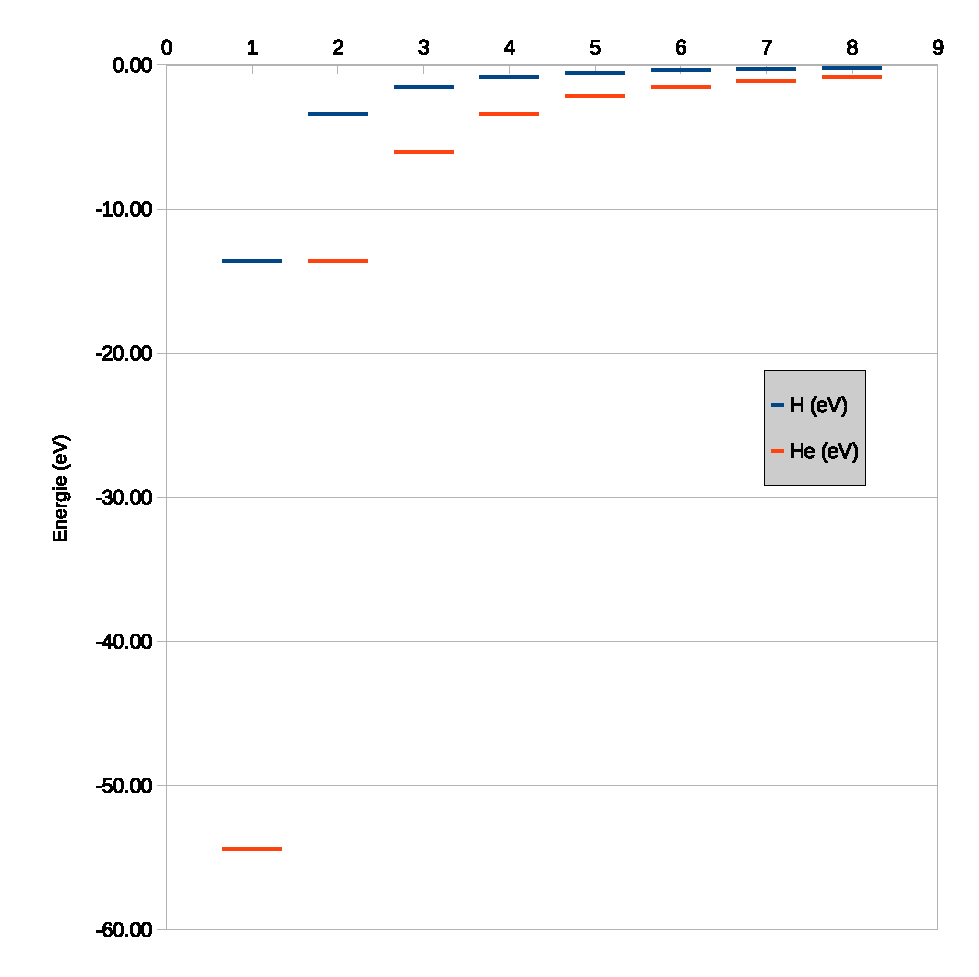
\includegraphics[width=1.0\textwidth]{figure/niveaux.eps}
\item Pour connaître le domaine dans lequel se trouve la série de Lyman, on calcule ses longueurs
d'onde maximales et minimales:\\
Longueur d'onde maximale : $n=2\rightarrow n=1$
\begin{align*}
\Delta E & =  \left|-13.6 ( \frac{1^2}{1^2} - \frac{1^2}{2^2} ) \right| \\
         & = 10.2 eV \\
\lambda_{max} & = \frac{hc}{\Delta E} \\
              & = \frac{6.626\times10^{-34} \times 3\times 10^8}{10.2\times1.602\times10^{-19}}\\
              & = 121,6 nm
\end{align*}
Longueur d'onde minimale : $n=\infty\rightarrow n=1$
\begin{align*}
\Delta E & = \left| -13.6 ( \frac{1^2}{1^2} - 0               ) \right| \\
         & = 13.6 eV \\
\lambda_{max} & = \frac{hc}{\Delta E} \\
              & = \frac{6.626\times10^{-34} \times 3\times 10^8}{13.6\times1.602\times10^{-19}}\\
              & = 91,2 nm
\end{align*}
Toutes les longueurs d'ondes de la série de Lyman se trouvent entre 91,2 et 121,6 nm, elles sont
donc toutes hors du visible.
\begin{itemize}
\item $400nm\rightarrow3,10 eV$
\item $800nm\rightarrow1,55 eV$
\item On calcule toutes les énergies de transition possibles et on cherche celles
qui se trouvent entre 3,10 et 1,55.\\
\begin{tabular}{lrrrrrr}\hline\hline
n & 1 & 2 & 3 & 4 & 5 & 6 \\\hline
He (eV) &-54.4 &-13.6 &-6.0 &-3.4 &-2.2 &-1.5 \\
\hline
$(n+1)\rightarrow n$   && 40.8 & 7.6 & \textbf{2.6} & 1.2 & 0.7 \\
$(n+2)\rightarrow n$&& & 48.4 & 10.2 & 3.9 & \textbf{1.9} \\
$(n+3)\rightarrow n$&& & & 51.0 & 11.4 & 4.5 \\
$(n+4)\rightarrow n$&& & & & 52.2 & 12.1 \\
$(n+5)\rightarrow n$&& & & & & 52.9 \\\hline\hline
\end{tabular}\\
Seules deux transitions sont dans le domaine du visible: $n: 4\rightarrow 3$ et $n: 6\rightarrow 4$
Ce sont des transitions d'un état excité vers un autre: elles sont peu probables donc difficiles
à observer.
\end{itemize}
\item Si on part de n=3 on peut faire les desexcitations suivantes:\\
\begin{tabular}{lll}
chemin 1: & $3\rightarrow 1$ \\
chemin 2: & $3\rightarrow 2$ & $2\rightarrow 1$ \\
\end{tabular}
\end{enumerate}
Il y aura donc 3 raies d'emission.\\
En partant de n=4, on a:\\
\begin{tabular}{llll}
chemin 1: & $4\rightarrow 1$ \\
chemin 2: & $4\rightarrow 2$ & $2\rightarrow 1$ \\
chemin 3: & $4\rightarrow 3$ & $3\rightarrow 1$ \\
chemin 4: & $4\rightarrow 3$ & $3\rightarrow 2$ & $2\rightarrow 1$ \\
\end{tabular}\\
Il y a 8 raies de desexcitations
\item La desexcitation $2\rightarrow 1$ se retrouve dans 2 chemins sur 4.
Donc 50\% des particules de départ l'emprunteront.
\subsection{Exercice 12}
\end{document}
